
\begin{figure}[t]
\centering
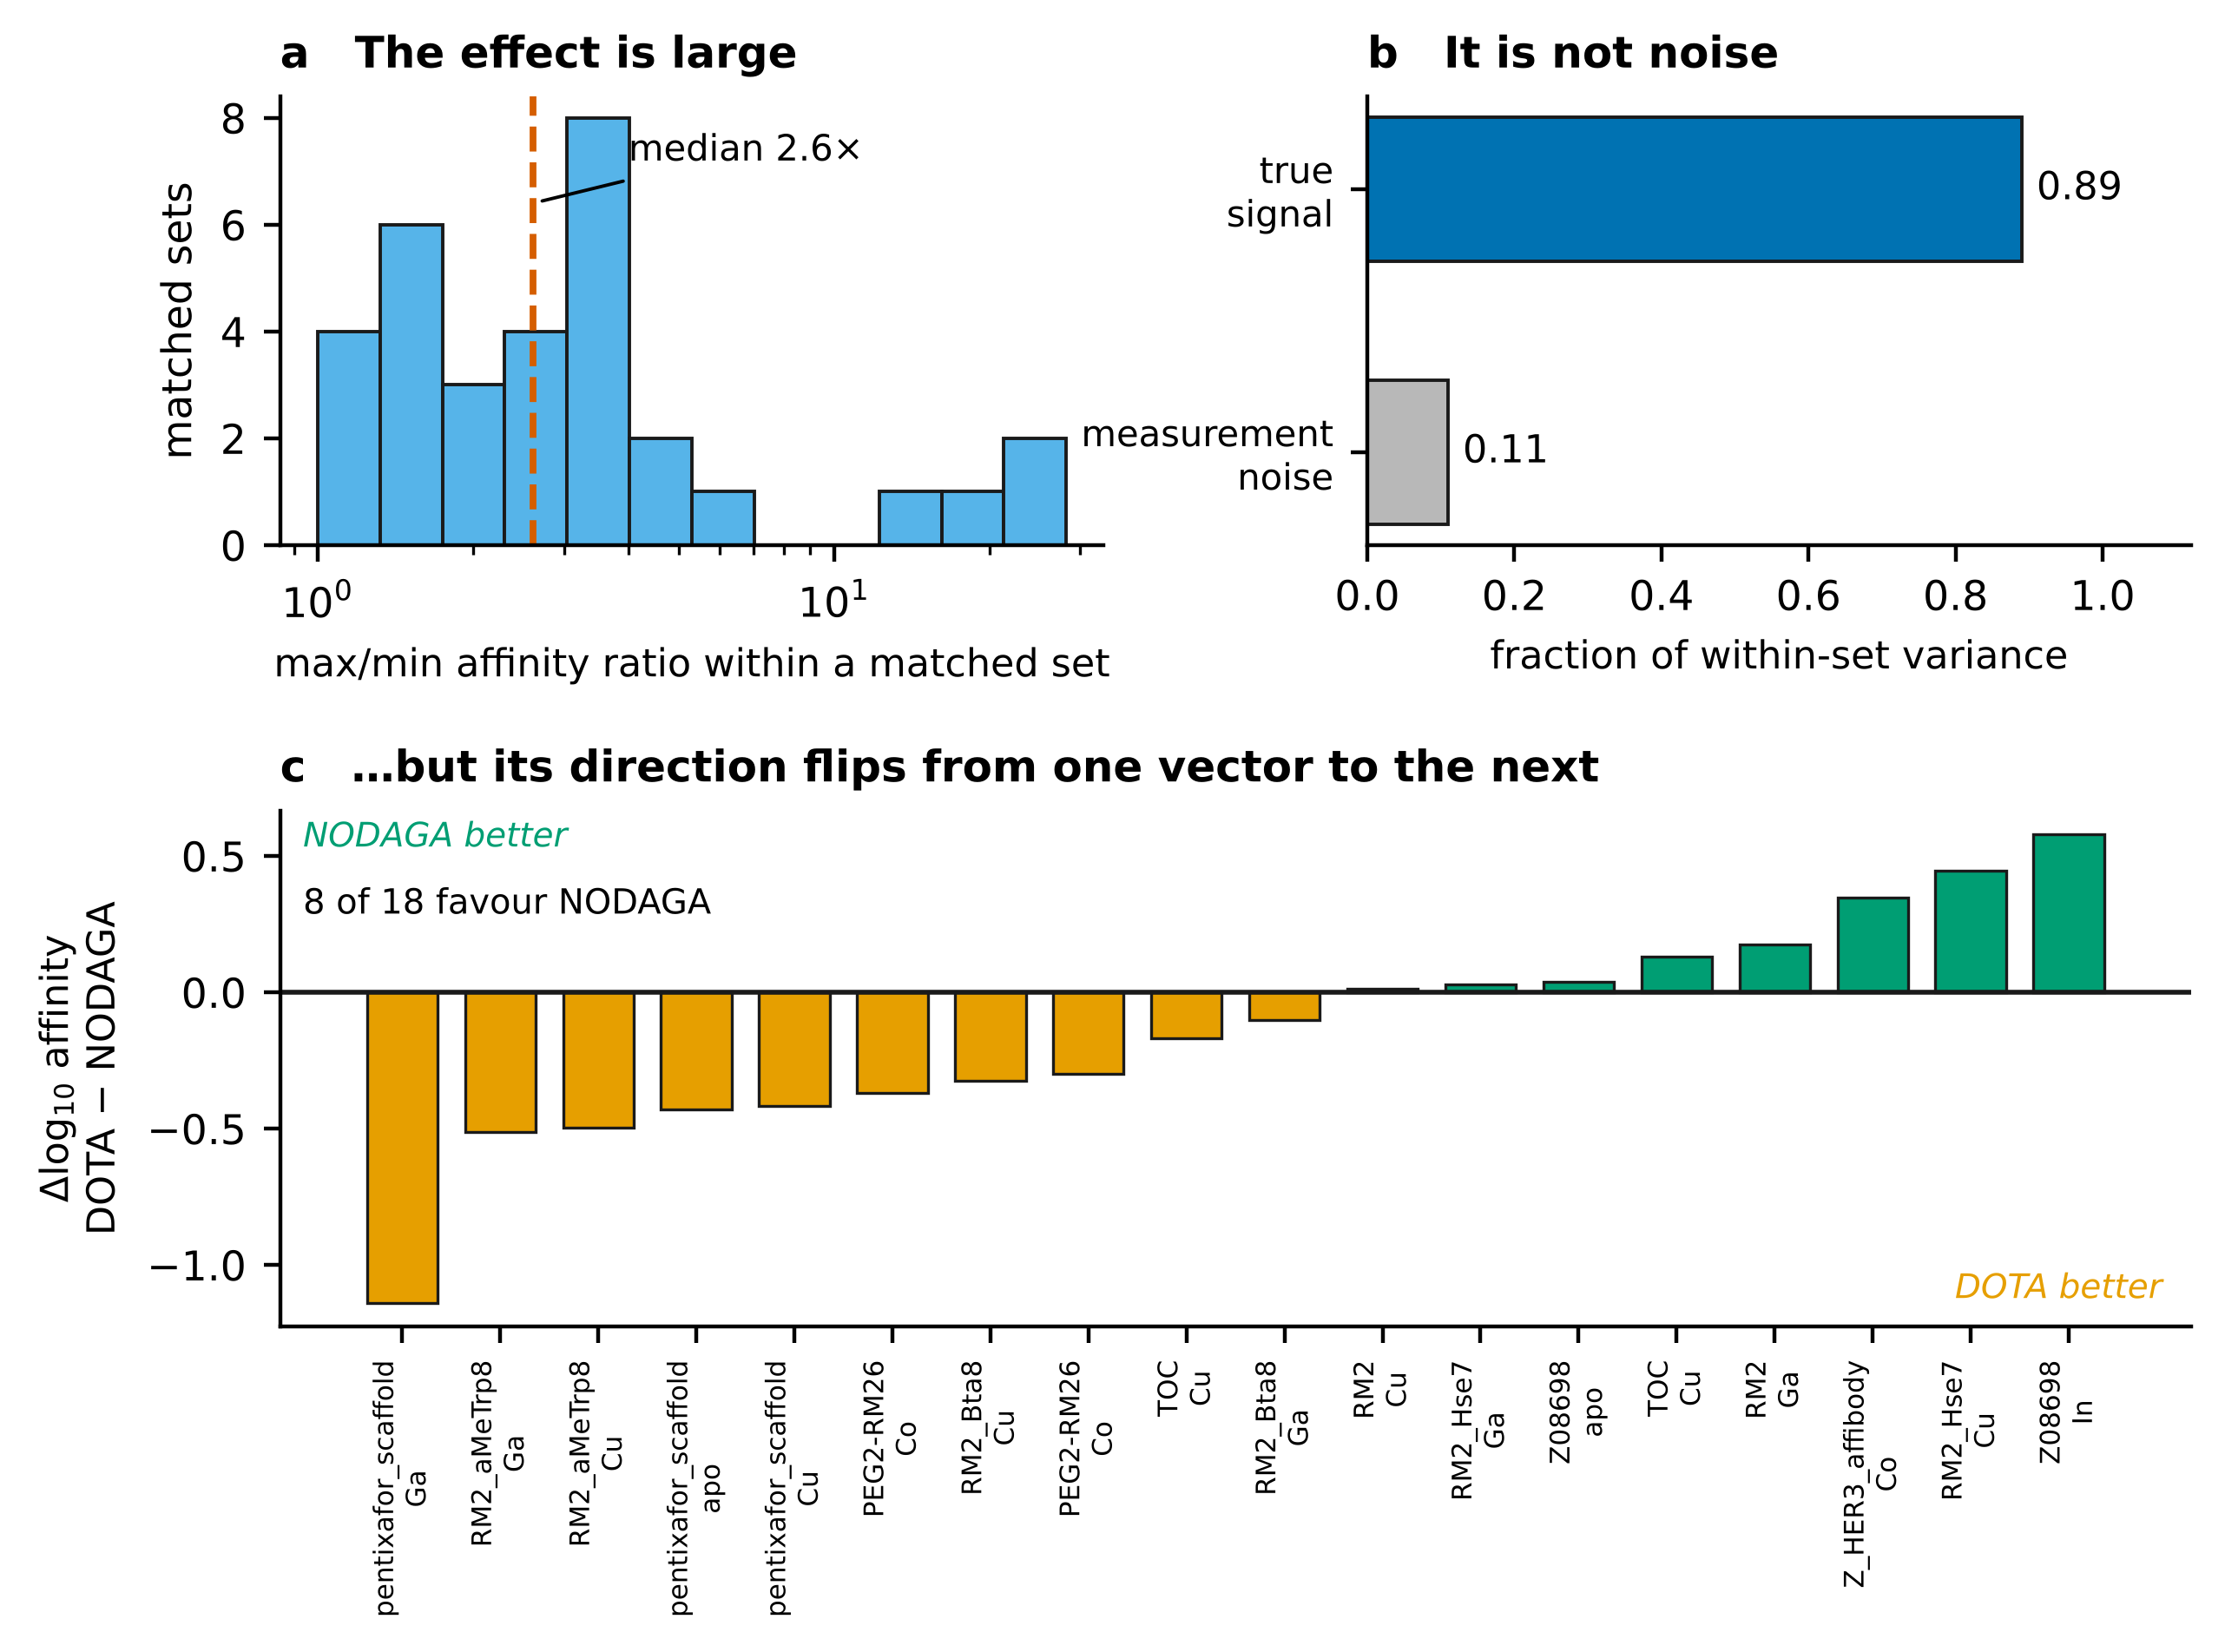
\includegraphics[width=\columnwidth]{Fig1.png}
\caption{\textbf{Chelate--vector coupling is large, is not noise, and reverses between vectors.} (\textbf{a}) Distribution of the maximum/minimum affinity ratio within each of 32 matched sets; dashed line, median 2.6-fold. (\textbf{b}) Decomposition of within-set variance into measurement error, propagated from reported standard deviations, and true signal. (\textbf{c}) Within-set difference in log$_{10}$ affinity between DOTA and NODAGA for all 18 sets containing both, labelled by vector and metal; bars above zero (green) mark sets in which NODAGA is the stronger binder, bars below zero (orange) those in which DOTA is. The direction reverses from one vector to the next, 8 of 18 favouring NODAGA.}
\label{fig:1}
\end{figure}

\begin{figure}[t]
\centering
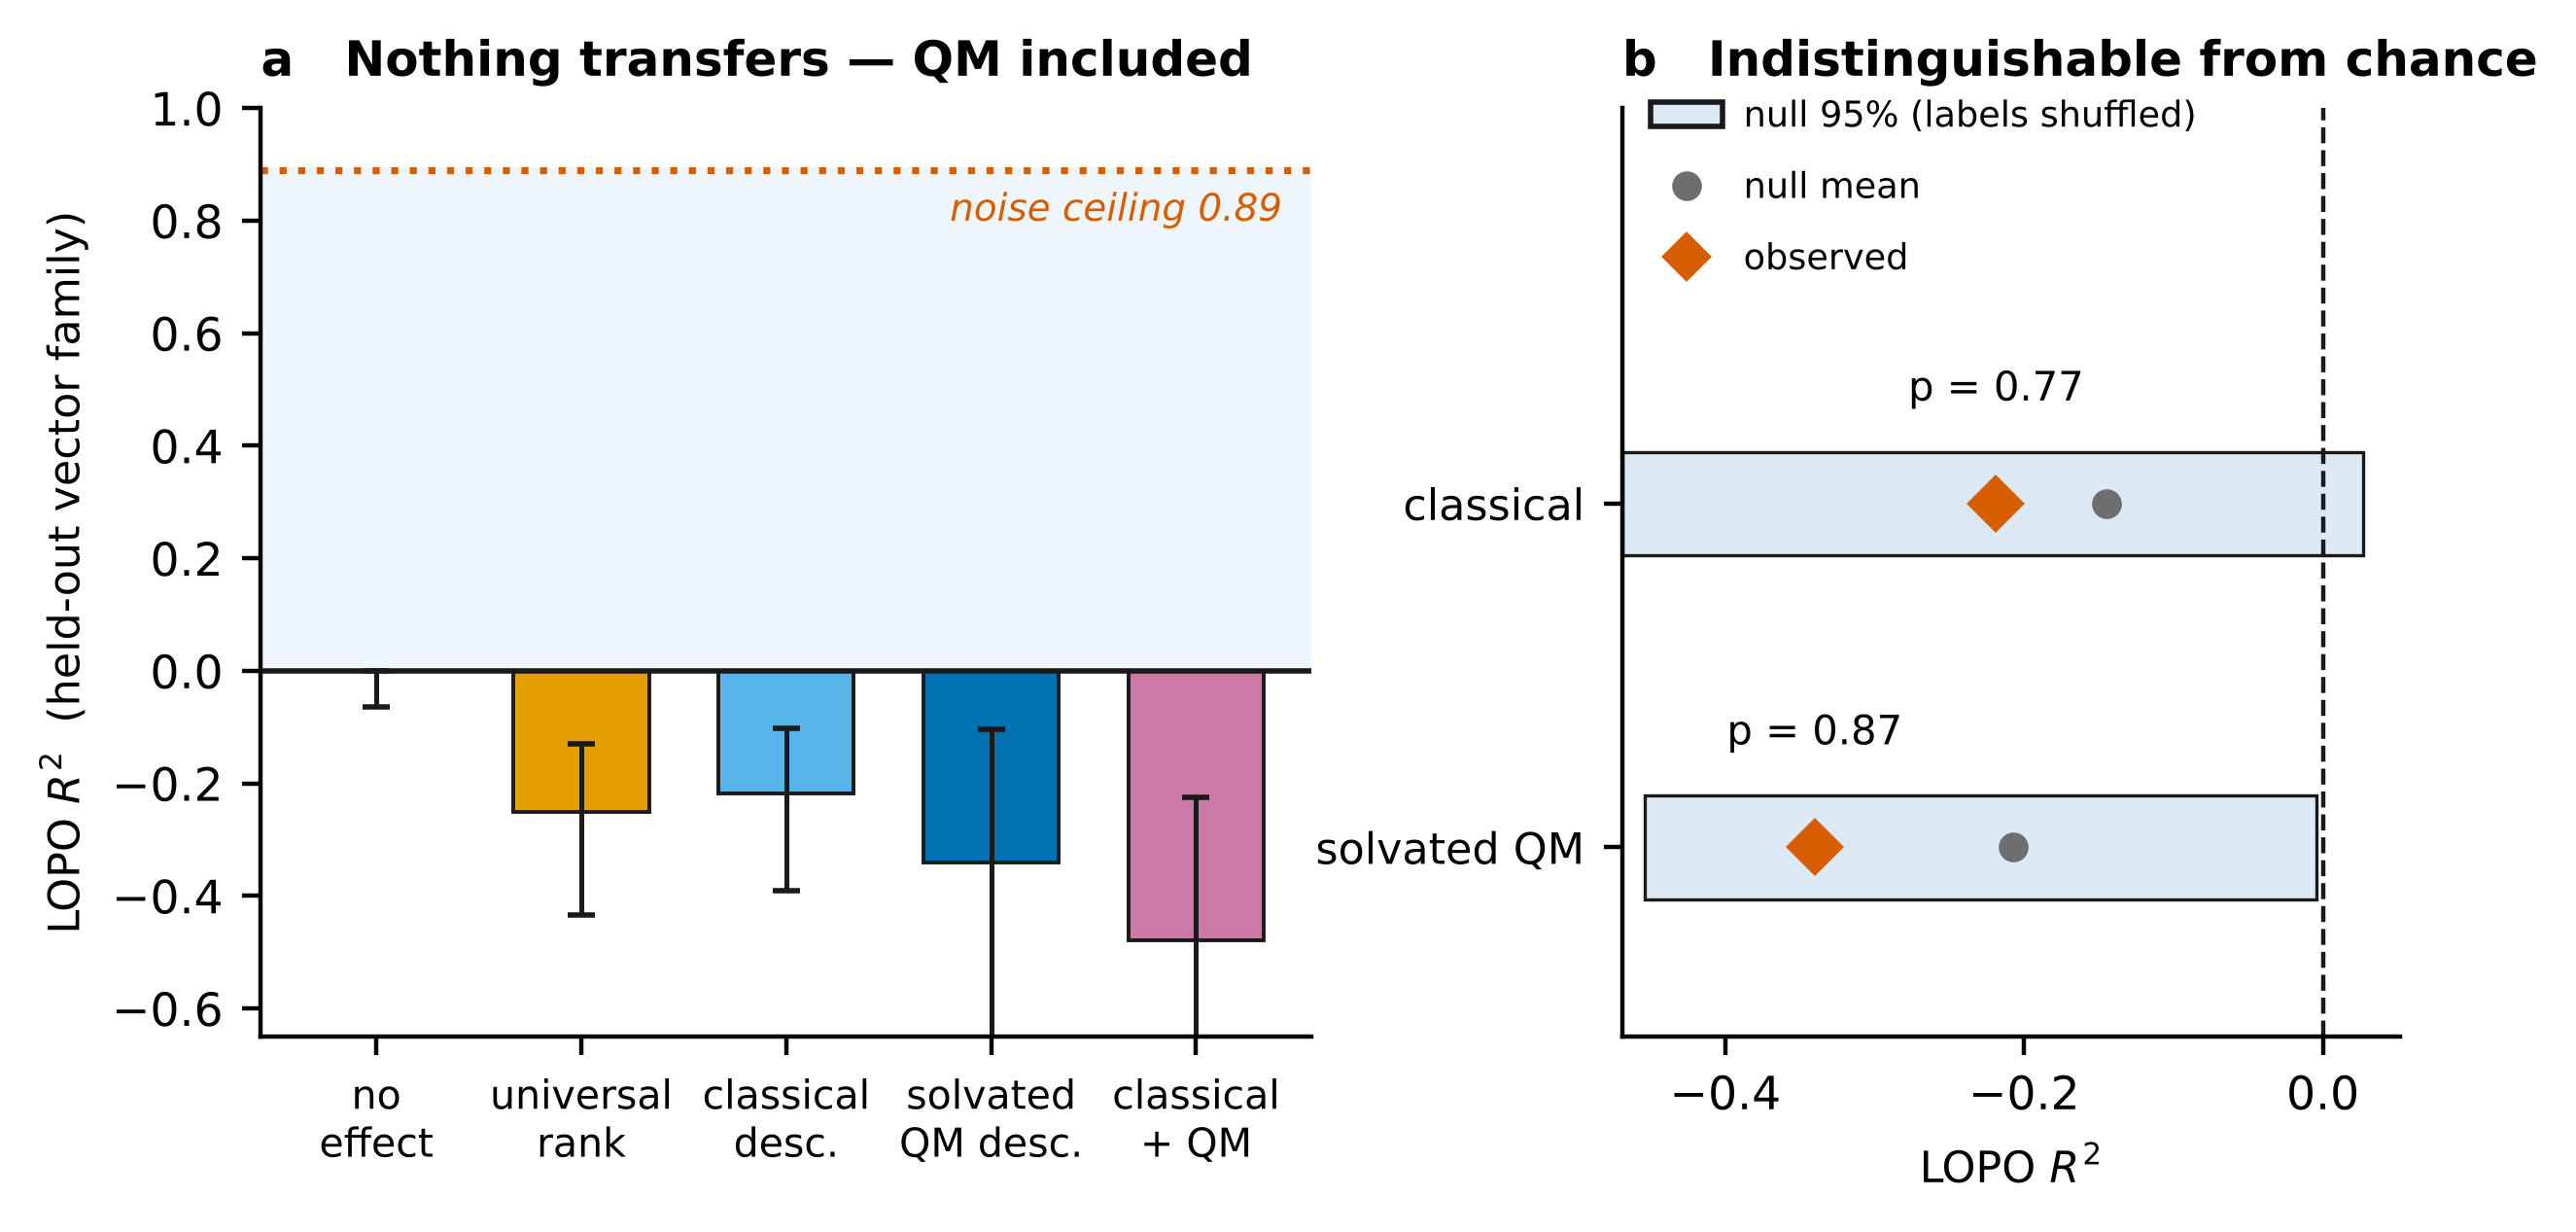
\includegraphics[width=\columnwidth]{Fig2.png}
\caption{\textbf{No descriptor set transfers to a held-out target family.} (\textbf{a}) Leave-one-target-family-out $R^2$ for five models ($n = 82$); error bars, 10\,000-sample bootstrap 95\% CI; shaded region, the range up to the measurement-noise ceiling of 0.890. (\textbf{b}) Observed LOPO $R^2$ (diamonds) against the null distribution from 2000 within-set label permutations (boxes, 95\% interval; circles, null mean).}
\label{fig:2}
\end{figure}

\begin{figure}[t]
\centering
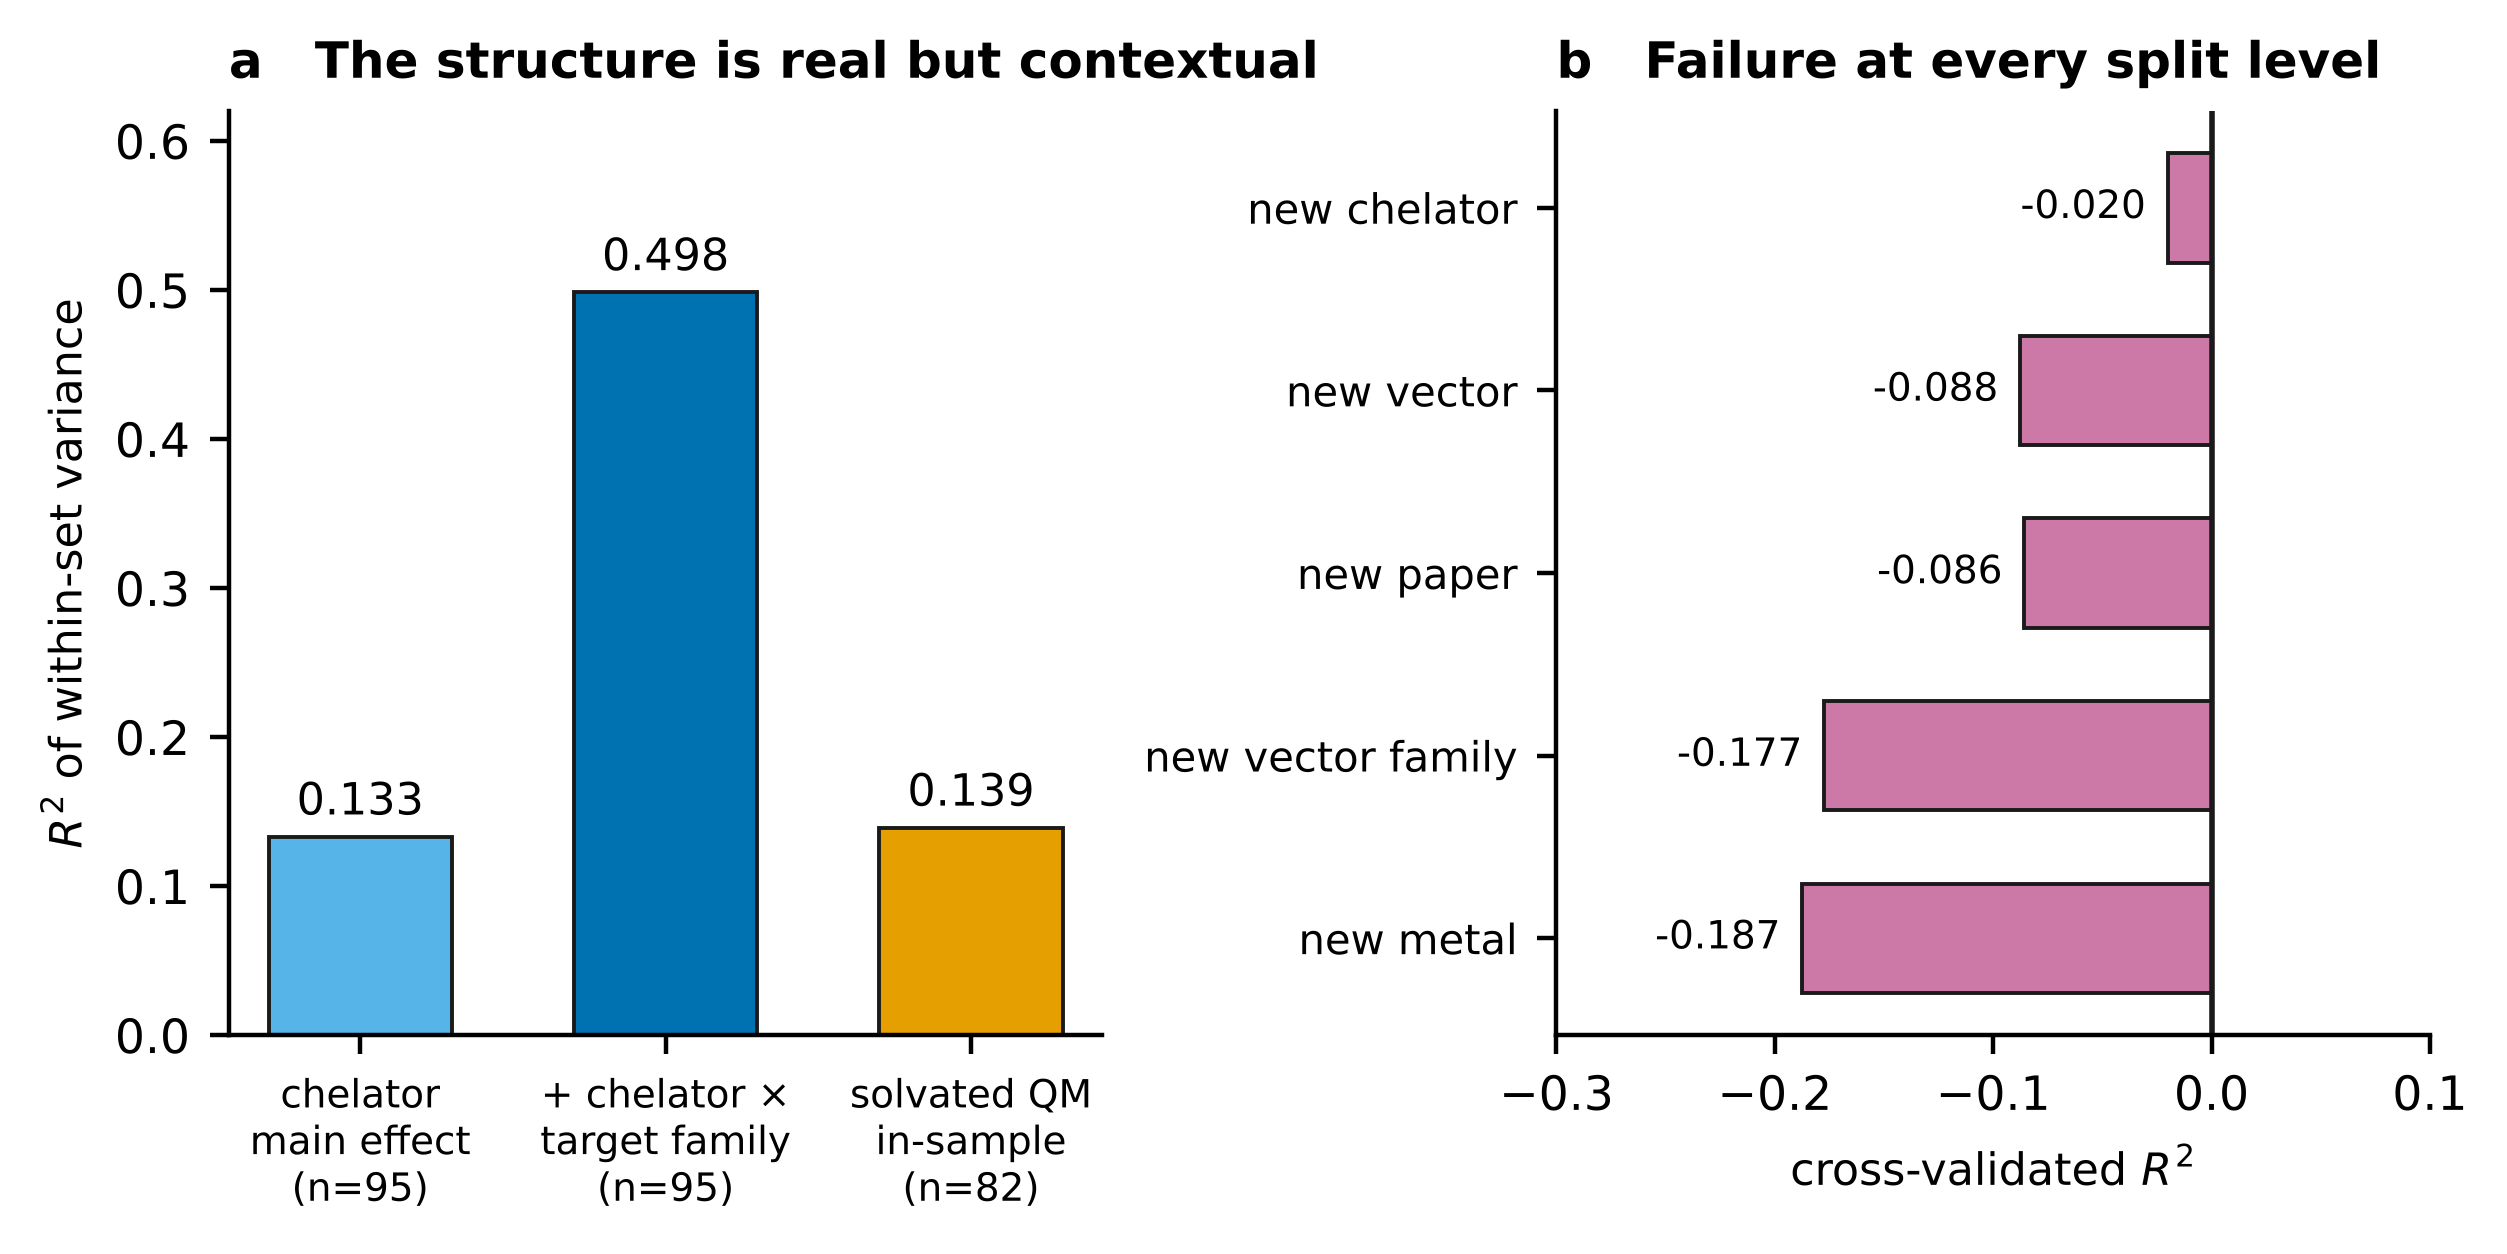
\includegraphics[width=\columnwidth]{Fig3.png}
\caption{\textbf{The effect is structured but contextual, and transfer fails at every level.} (\textbf{a}) Fraction of within-set variance explained by chelator alone and by chelator interacted with target family (full 95-row set), and by quantum-chemical descriptors fitted in sample (82-row subset). (\textbf{b}) Cross-validated $R^2$ under five held-out grouping schemes.}
\label{fig:3}
\end{figure}

\begin{figure*}[t]
\centering
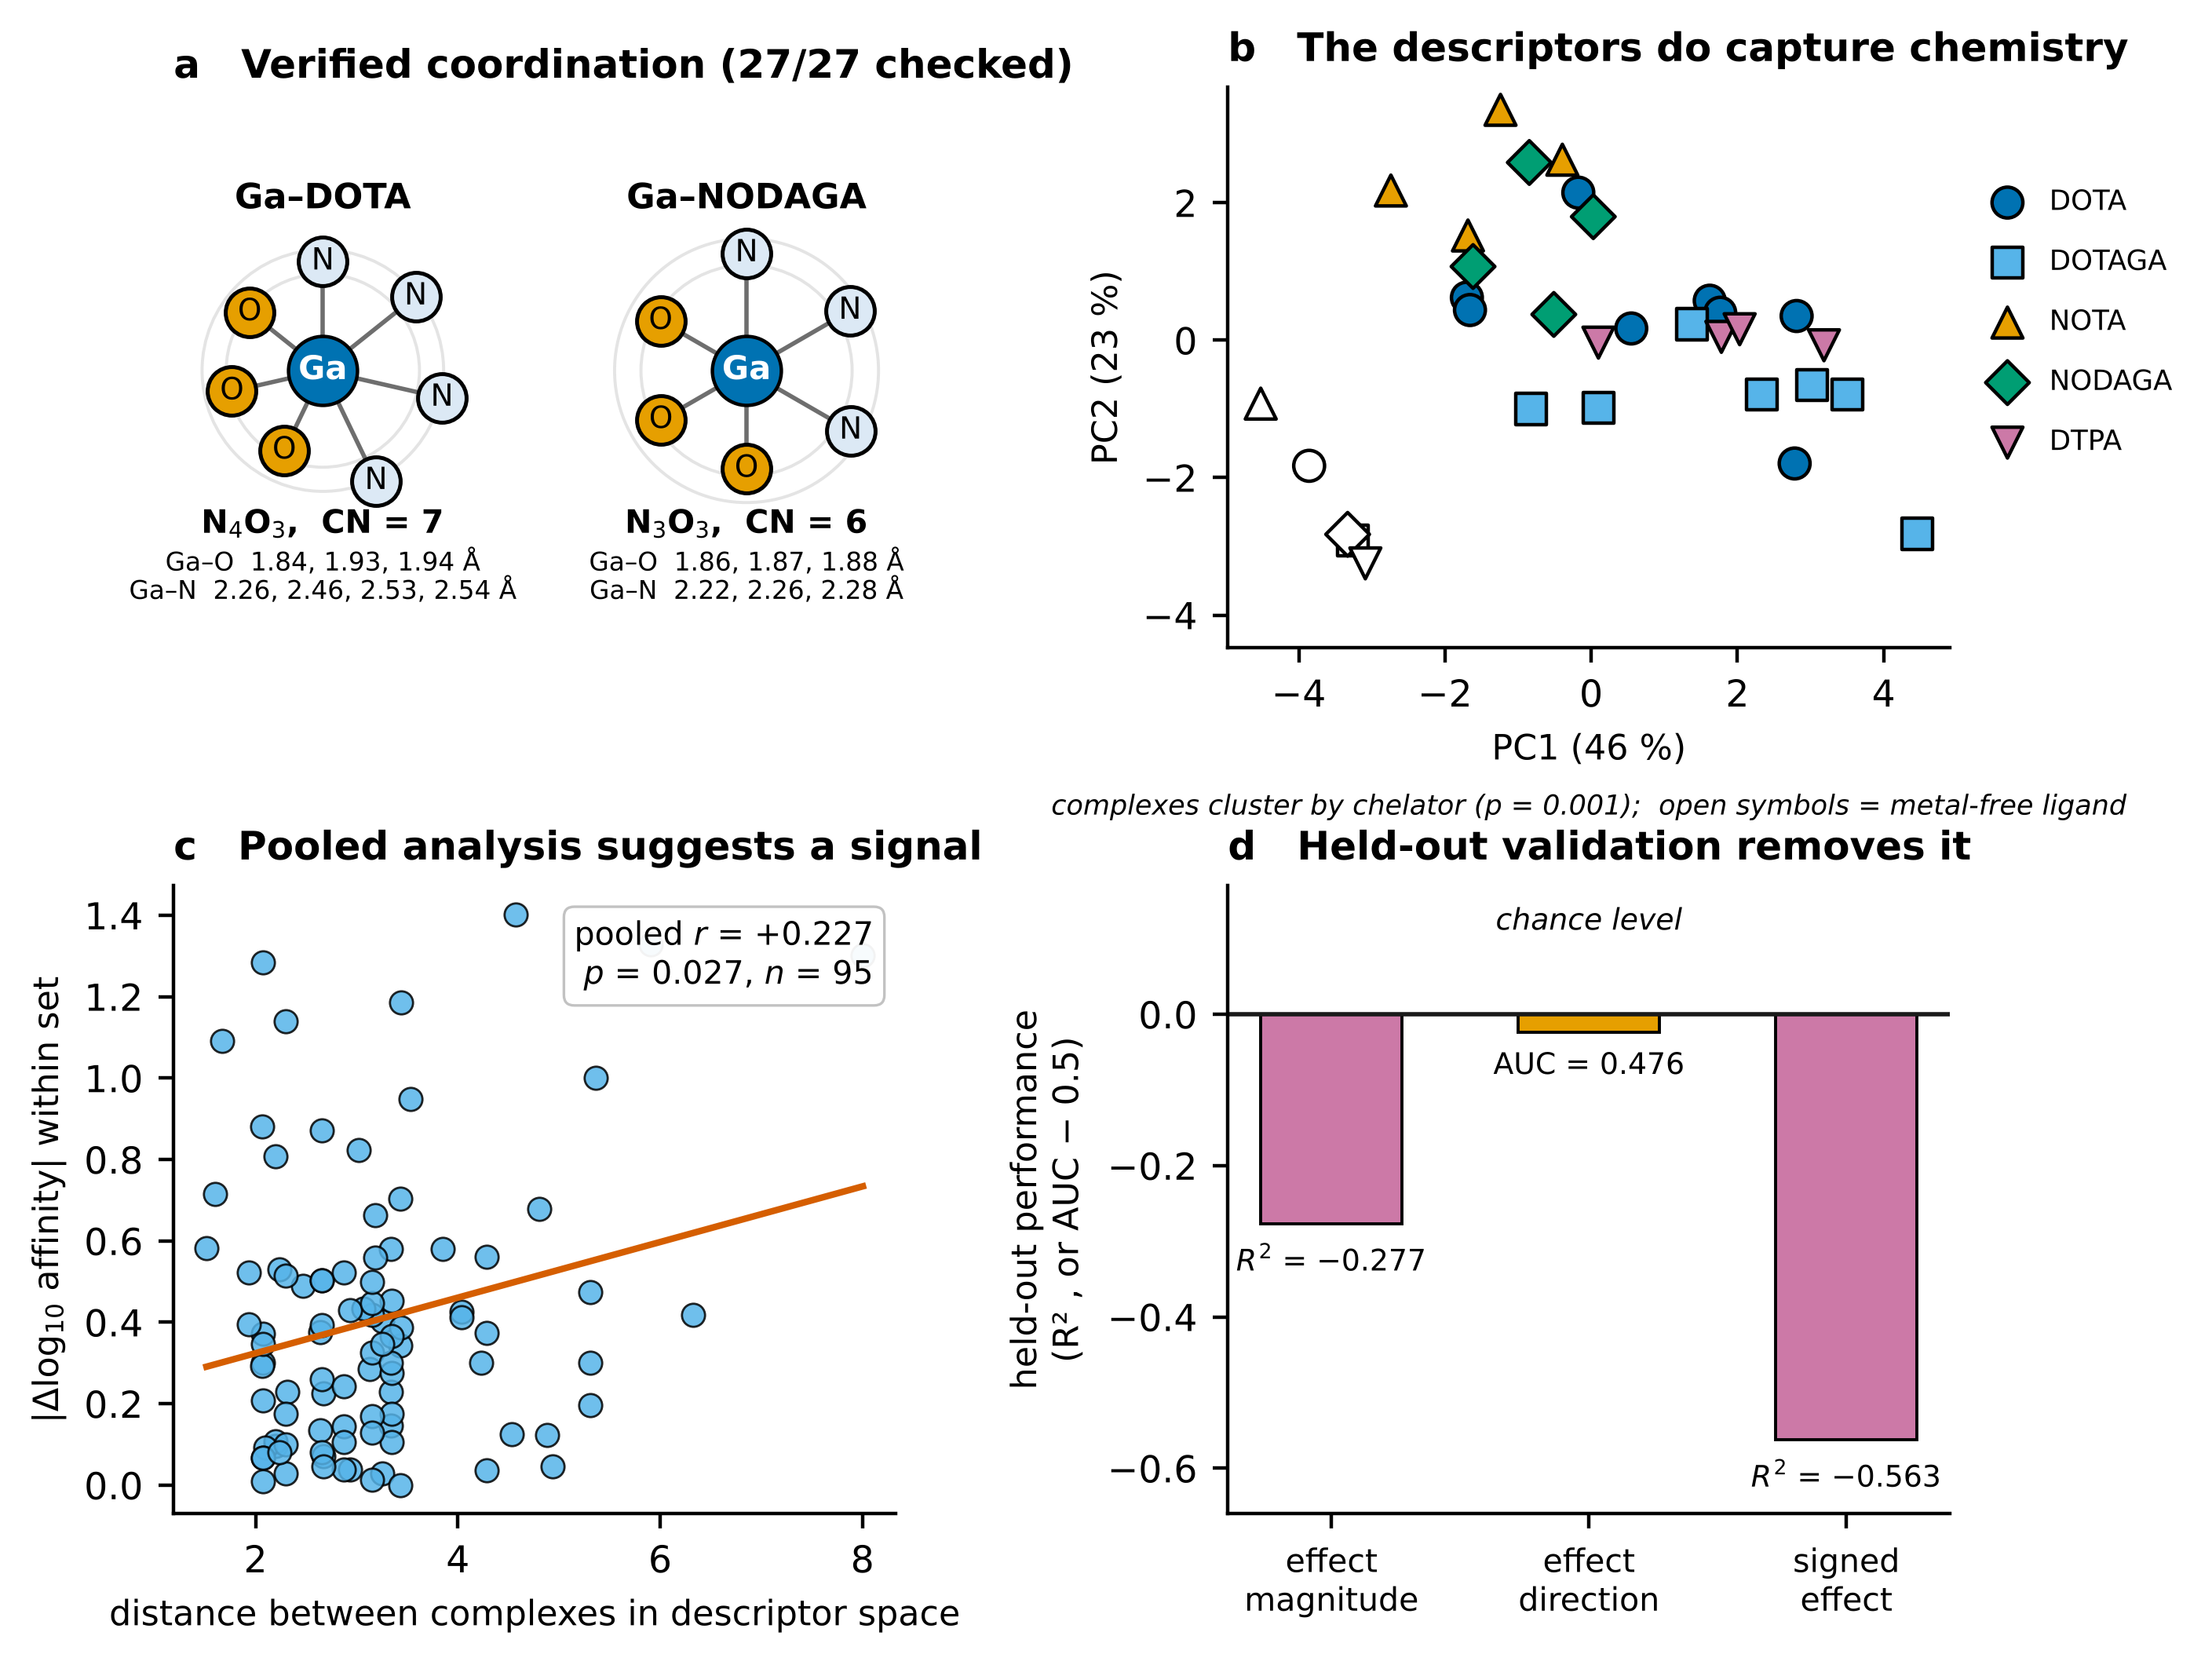
\includegraphics[width=0.86\textwidth]{Fig4.png}
\caption{\textbf{The descriptors are chemically sound, and the signal they appear to carry does not survive held-out validation.} (\textbf{a}) Coordination fingerprints of two optimised complexes, Ga--DOTA and Ga--NODAGA; donor atoms are placed at equal angles with the radius equal to the computed metal--donor distance. Coordination mode was verified against the known mode for every complex (27/27). (\textbf{b}) The 32 complexes in the first two principal components of the twelve descriptors; symbols denote chelator, open symbols the metal-free ligand. (\textbf{c}) Distance between two complexes in descriptor space against the magnitude of the affinity difference between them, pooled over all 95 within-set chelator pairs. (\textbf{d}) The same quantities under leave-one-target-family-out validation: magnitude, direction and the signed effect. Direction is shown as AUC $-$ 0.5 on the same axis and was evaluated on the antisymmetrised pair set, so that zero on this axis is chance by construction.}
\label{fig:4}
\end{figure*}
